\documentclass{article}
\usepackage{fancyvrb}
\usepackage{xcolor}
\usepackage{pygments}

\usepackage{polytexnic}
\begin{document}

\title{The Tau Manifesto}
\author{Michael Hartl}
\date{June 28, 2010}
\maketitle

\section{The most important number} % (fold)
\label{sec:the_most_important_number}

Welcome to the \emph{Tau Manifesto}. This manifesto is dedicated to one of the most important numbers in mathematics, perhaps \emph{the} most important number: the \emph{circle constant} relating the circumference of a circle to its linear dimension. For millennia, the circle has been considered the most perfect of shapes, and the circle constant captures the geometry of the circle in a single number. Surely, defining this number properly is a task that the great mathematicians of history should---nay, \emph{must}---have gotten right\ldots

Only they didn't.  As mathematician \href{http://www.math.utah.edu/~palais/}{Bob Palais} notes in his delightful article ``$\pi$ Is Wrong!'',\footnote{Palais, Robert. ``$\pi$ Is Wrong!'', \emph{The Mathematical Intelligencer}, Volume~23, Number~3, 2001, pp.~7--8. (``$\pi$ Is Wrong!'' is available online at \href{http://www.math.utah.edu/~palais/pi.html}{Bob Palais' pi page}.)} $\pi$ \emph{is wrong}. The traditional definition for the circle constant sets $\pi$ (pi) equal to the ratio of the circle's circumference to its diameter:\footnote{The symbol $\equiv$ means ``is defined as''.}


\[
  \pi \equiv \frac{C}{D} = 3.14159265\ldots
\]

\noindent Unfortunately, this definition is off by a factor of two in the denominator. Since a circle is the set of points a fixed distance---the \emph{radius}---from a given point, the most natural definition for the circle constant uses $r$ in place of $D$:

\[
  \mathrm{circle\ constant} = \frac{C}{r}
\]

Although he argues persuasively in favor of the above definition, even the plucky Professor Palais can't quite bring himself to take his idea seriously. Indeed, his initial inclination is to \emph{redefine} $\pi$ as

\[
  \pi \equiv \frac{C}{r}
\]

\noindent Given how deeply entrenched $\pi$ is in its current form, this redefinition is a complete nonstarter; it suggests, with a wistful tone, a ``wouldn't it have been nice if\ldots'' sentiment that has no chance of any real-world usage---thereby \emph{approaching} the truth but stopping short when the implications become too uncomfortable.\footnote{George Orwell called this phenomenon \href{http://en.wikipedia.org/wiki/Crimestop}{\emph{crimestop}}.} Of course, using $\pi$ in the manner above would be hopelessly confusing, so ultimately Dr. Palais does introduce a separate symbol for the circle constant, which he calls ``one turn''.  As we'll see, the description is prescient, but the symbol, lamentably, is absurd (\hyperref[fig:palais-tau]{Figure~}\ref{fig:palais-tau}).\footnote{Why propose an absurd symbol that has no chance of ever being used in a serious context? As I said: \href{http://en.wikipedia.org/wiki/Crimestop}{\emph{crimestop}}.}


\begin{figure}
\begin{center}

\includegraphics{images/figures/palais-tau.png}
\end{center}
\caption{The absurd symbol used for the circle constant in ``$\pi$ Is Wrong!''.\label{fig:palais-tau}}
\end{figure}

The \emph{Tau Manifesto} is dedicated to the following proposition: The proper response to ``$\pi$ is wrong'' is ``No, \emph{really}.'' And the true circle constant deserves a proper name. The \emph{Tau Manifesto} proposes that this name---as I hope you will not be surprised to learn---should be the Greek letter $\tau$ (tau):

\[
  \tau \equiv \frac{C}{r} = 6.2831853071796586\ldots
\]

\noindent This symbol is neither confusing nor absurd, and (as we'll see in \hyperref[sec:why_tau]{Section~}\ref{sec:why_tau}) there are some powerful arguments in its favor. Moreover, regardless of how many converts $\tau$ ultimately gains, no one can stop \emph{us} from using it. For proof, simply read on.


 \subsection{A powerful enemy} % (fold)

Before proceeding with the demonstration that $\tau$ is the natural choice for the circle constant, let us first acknowledge what we are up against---for there is a powerful conspiracy, centuries old, determined to propagate pro-$\pi$ propaganda. Entire \href{http://www.amazon.com/exec/obidos/ISBN=0802713327/parallaxproductiA/}{books} \href{http://www.amazon.com/Pi-Sky-Counting-Thinking-Being/dp/0198539568}{are} \href{http://www.amazon.com/exec/obidos/ISBN=0312381859/parallaxproductiA/}{written} extolling the virtues of $\pi$. I mean, \href{http://www.amazon.com/exec/obidos/ISBN=0387989463/parallaxproductiA/}{\emph{books}}\emph{!} And $\pi$ perfidy has captured even the highest levels of geekdom; for example, for the 2010 ``$\pi$ Day'' celebration (taking place annually on March~14), \href{http://www.google.com/}{Google} \emph{changed its logo} to honor $\pi$  (\hyperref[fig:google-pi-day]{Figure~}\ref{fig:google-pi-day}).  Meanwhile, some people memorize dozens, hundreds, even \emph{thousands} of digits of this mystical number. What kind of sad sack memorizes dozens of digits of $\pi$ (\hyperref[fig:michael_hartl]{Figure~}\ref{fig:michael_hartl})?

\begin{figure}
\begin{center}
\image{images/figures/google-pi-day.gif}
\end{center}
\caption{The Google logo on March 14, 2010.\label{fig:google-pi-day}}
\end{figure}

\begin{figure}
\begin{center}
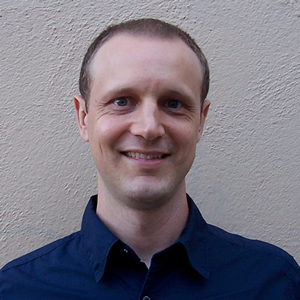
\includegraphics{images/figures/michael_hartl.jpg}
\end{center}
\caption{This poor bastard once memorized $\pi$ to 50 decimal places.\label{fig:michael_hartl}}
\end{figure}

Truly, we warriors of the $\tau$ face a mighty opponent. And yet, we have a powerful ally---for the truth is on our side.

% section the_most_important_number (end)

\section{The nature of angle} % (fold)

Look through 

and you see...

But the best demonstration ...

Students of trigonometry learn special angles (\hyperref[fig:degree-angles]{Figure~}\ref{fig:degree-angles}).

\begin{figure}
\begin{center}
\image{images/figures/degree-angles.png}
\end{center}
\caption{Some important angles, in degrees.\label{fig:degree-angles}}
\end{figure}

Degrees break circles arbitrarily into 360 equal parts. More natural is to note that, since 

 \subsection{Radian angle measure} % (fold)
 \label{sec:radian_angle_measure}
 
 % subsection radian_angle_measure (end)

\begin{figure}
\begin{center}
\image{images/figures/angle-arclength.png}
\end{center}
\caption{The arclengths $s$ and radii $r$ differ, but since $s\propto r$ the ratios are the same.\label{fig:angle-arclength}}
\end{figure}

The arclengths differ, but the \emph{ratio} of the arclength to the radius is the same for each. This suggests the following definition of \emph{radian angle measure}:

\[ \theta = \frac{s}{r} \]

If you recall high-school trig, you probably have the special angles shown in \hyperref[fig:pi-angles]{Figure~}\ref{fig:pi-angles} floating around in your brain. I call this system of measure $\pi$-radians to emphasize that they are written in terms of $\pi$.

\begin{figure}
\begin{center}
\image{images/figures/pi-angles.png}
\end{center}
\caption{Some important angles, in $\pi$-radians.\label{fig:pi-angles}}
\end{figure}

We now begin to see just how stupid $\pi$ is. For a moment's reflection shows that the so-called ``special'' angles are simply  \emph{rational fractions} of a full circle, as shown in \hyperref[fig:angle-fractions]{Figure~}\ref{fig:angle-fractions}.

\begin{figure}
\begin{center}
\image{images/figures/angle-fractions.png}
\end{center}
\caption{The ``important'' angles are rational fractions of a full circle.\label{fig:angle-fractions}}
\end{figure}

\noindent We can now revisit the definition of radian angle measure, noting that the arclength~\emph{s} for an angle representing some fraction~\emph{f} of a circle is simply that same fraction of the circumference:

\[ \theta = \frac{s}{r} = \frac{fC}{r} =  f\left(\frac{C}{r}\right) \equiv f\tau \]

\noindent Notice how naturally $\tau$ falls out of this analysis. The resulting diagram of angles---shown in \hyperref[fig:tau-angles]{Figure~}\ref{fig:tau-angles}---is a powerful argument in favor of $\tau$.
Indeed, upon comparing \hyperref[fig:tau-angles]{Figure~}\ref{fig:tau-angles} and \hyperref[fig:angle-fractions]{Figure~}\ref{fig:angle-fractions}, I consider it decisive.

\begin{figure}
\begin{center}
\image{images/figures/tau-angles.png}
\end{center}
\caption{Some important angles, in radians.\label{fig:tau-angles}}
\end{figure}

One turn.

No memorization.

To those who maintain that it ``doesn't matter'' whether we use $\pi$ or $\tau$ in trigonometry, I simply ask you to view \hyperref[fig:pi-angles]{Figure~}\ref{fig:pi-angles} and \hyperref[fig:tau-angles]{Figure~}\ref{fig:tau-angles} through the eyes of a child. You will see that, from the perspective of a beginner, \emph{using $\pi$ instead of $\tau$ is a pedagogical disaster.}

  \subsection{The circle functions} % (fold)
  \label{sec:the_circle_functions}

\begin{figure}
\begin{center}
\image{images/figures/sine-with-tau.png}
\end{center}
\caption{Important points for $\sin\theta$ in terms of the period $T$.\label{fig:sine-with-tau}}
\end{figure}

Lorem ipsum dolor sit amet, consectetur adipisicing elit, sed do eiusmod tempor incididunt ut labore et dolore magna aliqua. Ut enim ad minim veniam, quis nostrud exercitation ullamco laboris nisi ut aliquip ex ea commodo consequat. Duis aute irure dolor in reprehenderit in voluptate velit esse cillum dolore eu fugiat nulla pariatur. Excepteur sint occaecat cupidatat non proident, sunt in culpa qui officia deserunt mollit anim id est laborum.
  
  % subsection the_circle_functions (end)

% section radian_angle_measure (end)

Can write

\[ e^{i\theta} = \cos\theta + i\sin\theta \]

Evaluating at $\theta = \tau$ yields \emph{Euler's formula}:

\[ e^{i\tau} = 1 \]


In words, this equation makes the following fundamental observation: 

\begin{center}
\emph{The exponential of the imaginary unit times the circle constant is unity.} 
\end{center}

Since complex exponentials correspond to rotations in the complex plane, this can also be stated as follows:

\begin{center}
\emph{The complex exponential of the circle constant is one turn.}
\end{center}

\noindent As in the case of radian angle measure, we see how natural the association is between $\tau$ and one turn of a circle.


Of course, Euler's formula is traditionally written in terms of $\pi$:


\[ e^{i\pi} = -1 \]

\noindent But that minus sign is so ugly that the formula is almost always rearranged immediately,\footnote{Where does that minus sign come from? And why does the equation sometimes called ``the most amazing equation in mathematics'' need rearranging? It's almost as if these things are trying to tell us something\ldots} yielding

\[ e^{i\pi} + 1 = 0 \]

\noindent At this point, the expositor usually makes some grandiose statement about how Euler's formula relates $0$, $1$, $e$, $i$, and $\pi$---sometimes called the ``five most important numbers of mathematics''. Alert readers might then complain that Euler's formula with $\tau$ relates only four of those five. For any such whiners out there, I offer this:

\[ e^{i\tau} + 0 = 1 \]

\noindent So there.

\section{Why tau?} % (fold)
\label{sec:why_tau}

Having 

Of course, there's no need to justify introducing a new variable; there's no arguing with the statement ``Let $\tau = 2\pi$.'' On the other hand, we could as well say ``Let $\alpha = 2\pi$'', but for a constant as fundamental as $\tau$ it would be nice to have some deeper reasons for our choice. Let me therefore offer the following three key arguments:

\begin{enumerate}
  \item \emph{$\tau$ is available.} \\ Although $\tau$ is used for, e.g., \emph{strain} in mechanical engineering and \emph{proper time} in special and general relativity, there is no universal conflicting usage.\footnote{Minor clashes are OK; after all, physicists manage to use $e$ both for the natural number and for the charge on an electron without causing apparent harm.} 
  
  \item \emph{$\tau$ resembles $\pi$.} \\ $\tau$ is typographically similar to $\pi$, thereby evoking the same notion of a circle constant.\footnote{Unfortunately, the number of ``legs'' isn't quite right: it would be poetic if we could write $\pi = 2\tau$, but it wasn't meant to be. Of course, in that case $\pi$ would have the right definition, and we wouldn't have this manifesto.}
  
  \item \emph{$\tau$ is one turn.} \\ We have seen that, geometrically speaking, $\tau$ represents one \emph{turn} of a circle. In this context, consider that the root of the English word ``turn'' is the Greek word for ``lathe'', \emph{tornos}---or, as the Greeks would put it: \[ \tau \acute{o}\rho\nu o\varsigma \] \noindent Looking at the first letter of that Greek lathe, I'm going to go out on a limb here and say: \href{http://en.wikipedia.org/wiki/Q.E.D.}{\emph{quod erat demonstrandum}}.
\end{enumerate}



\section{The coup de gr\^{a}ce} % (fold)
\label{sec:circular_area}

\[ A = \pi r^2 \]


Seems like the exception, but is really the \emph{coup de gr\^{a}ce}.

\[ v \propto t \]

\[ v = g t \]

\[ y = \int_0^t gt\,dt = \textstyle{\frac{1}{2}} gt^2 \]


\[ F \propto x \]

\[ F = k x \]

\[ U = \int_0^x kx\,dx = \textstyle{\frac{1}{2}} kx^2 \]

\[ F \propto a \]

\[ F = m a \]

\[ K = \int ma\,dx = \int m\,\frac{dv}{dt}\,dx = \int m\, \frac{dx}{dt}\,dv = \int_0^v mv\,dv = \textstyle{\frac{1}{2}} mv^2 \]


\begin{figure}
\begin{center}
\image{images/figures/circular-area.png}
\end{center}
\caption{Calculating the area of a circle using circular rings.\label{fig:circular-area}}
\end{figure}

\[ dA = C\,dr \]

\noindent But for a circle the circumference is proportional to the radius:

\[ C \propto r \]

\noindent The constant of proportionality is $\tau$:

\[ C = \tau r \]

\noindent The area of the full circle can then be calculated by integrating:

\[ A = \int_0^r C\,dr = \int_0^r \tau r\,dr = \textstyle{\frac{1}{2}} \tau r^2 \]




% section circular_area (end)

\section{Puns}

We come now to the final objection: ``What about puns?'', I hear you cry. I know, I know, ``$\pi$ in the sky'' is so very clever. And yet, $\tau$ itself is pregnant with possibilities. After all, once you have accepted $\tau$ism, you will become a $\tau$ist like me. It is not $\tau$ that is a piece of $\pi$, but $\pi$ that is a piece of $\tau$---half~$\tau$, to be exact. This is the true nature of the~$\tau$.

\section{Conclusion}

Mechanical substitution.

We are followers of the $\tau$, and June 28---$\tau$ Day---is $\tau$ism's holy day.\footnote{Indeed, 6/28 is a \emph{perfect} day---for 6 and 28 are the first two \href{http://en.wikipedia.org/wiki/Perfect_number}{\emph{perfect numbers}}.} I hope you will join us in celebrating!

\\

\textbf{About the author}

\emph{Tau Manifesto} author \href{http://www.michaelhartl.com/}{Michael Hartl} is an educator and entrepreneur. An experienced programmer, he is currently working on the  \href{http://www.railstutorial.org/}{Ruby on Rails Tutorial} project, which teaches web development using \href{http://www.rubyonrails.org/}{Ruby on Rails}. Previously, he taught theoretical and computational physics at the \href{http://www.caltech.edu/}{California Institute of Technology}, where he received the Lifetime Achievement Award for Excellence in Teaching. Michael knows 51 digits of $\pi$---i.e., fifty decimal places---approximately 48 more than \href{http://en.wikipedia.org/wiki/Matt_Groening}{Matt Groening}. He is now working on memorizing 53 digits of $\tau$.\footnote{It doesn't round off right if you truncate after 52 digits. But you probably figured that out already.}
\end{document}

